\tab Una dintre caracteristicele principale a unui \textbf{VCS} este faptul ca
ne permite sa revenim la o versiune mai veche. Aceasta poate fi efectuata cu ajutorul
comenzii \textbf{git reset --TYPE "codul comitului"}. Exista diferenta intre 
\textbf{--soft} si \textbf{--hard} , cind facem soft reset indexurile ramin neschimbate.
Iar in cazul cind facem hard reset , pierdem indexurile.
\\
\\
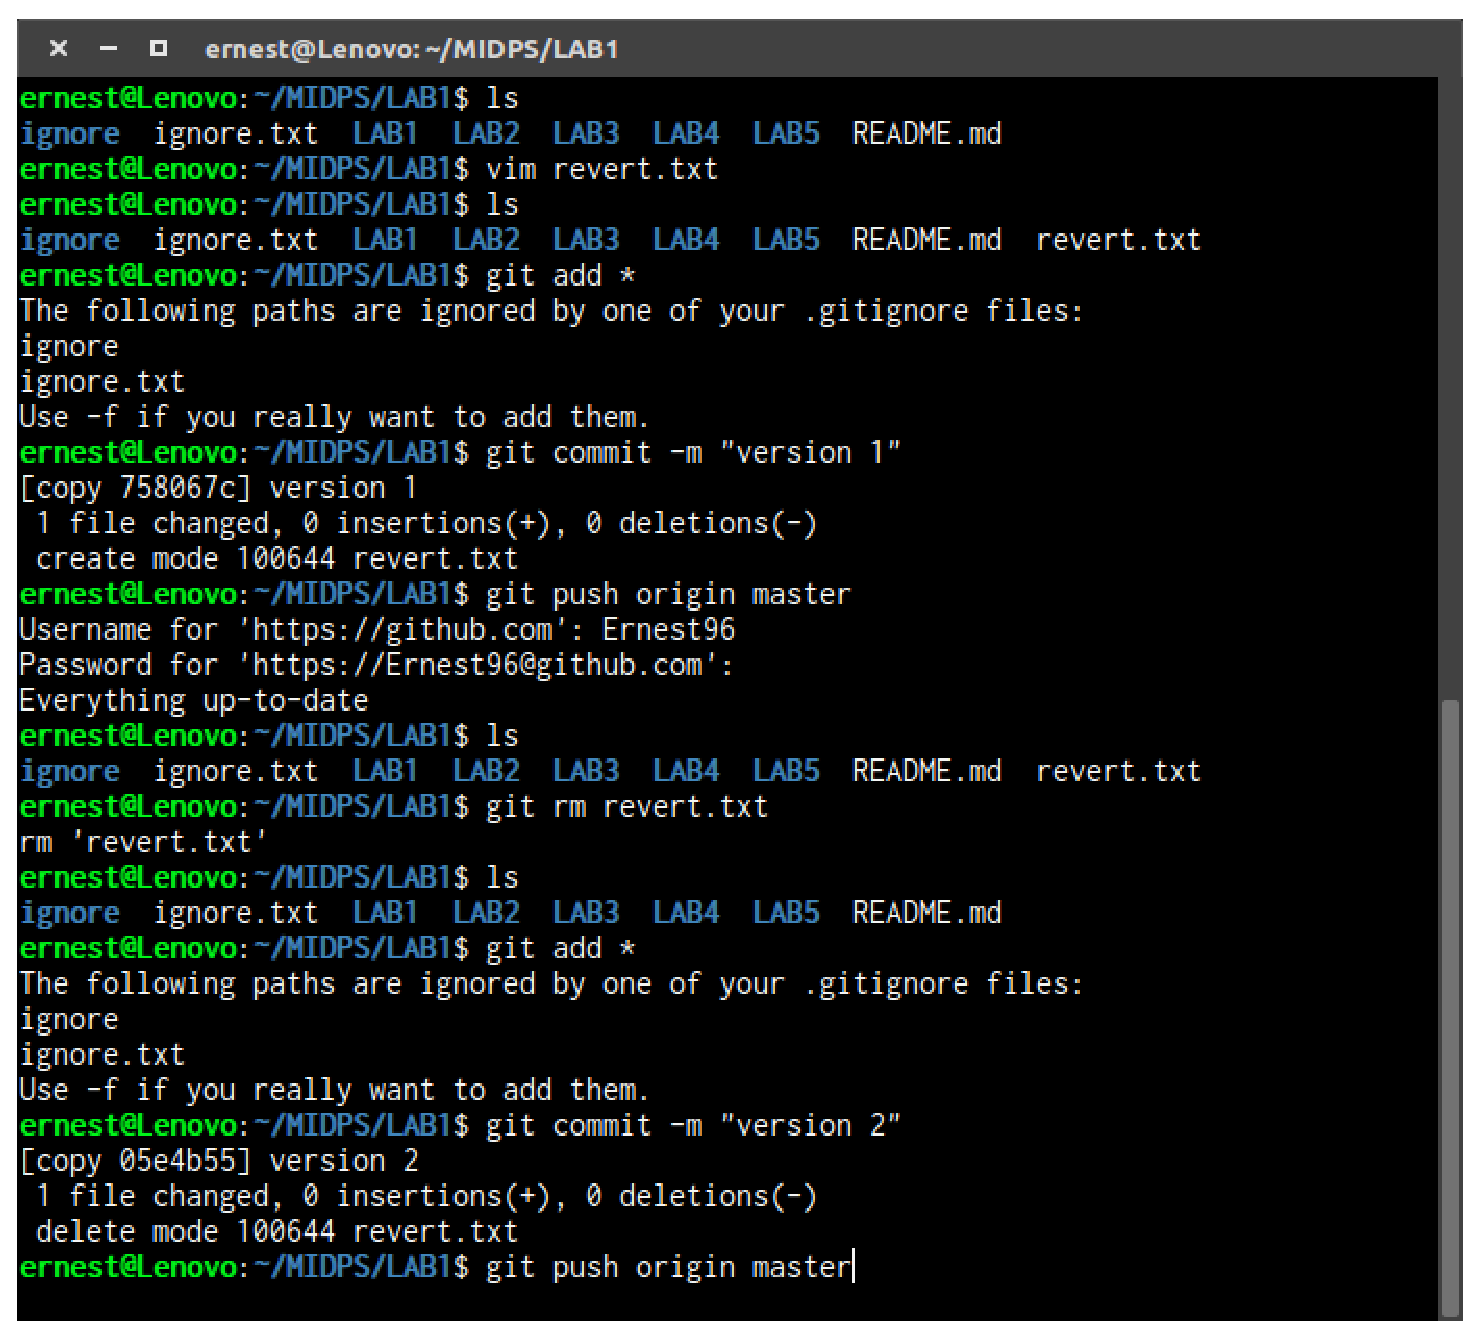
\includegraphics[width=\textwidth]{7.eps}
\\
\\
Dupa cum observam cind am facut commit, s-au ignorat fisierele incluse in .gitignore.
\clearpage
\tab Am creat un fisier nou revert.txt in versiunea 1. Dupa care l-am sters si am facut
commit la versiunea 2 in care am sters fisierul revert.txt dorim sa revenim la versiunea1. La inceput vom lansa comanda \textbf{git --log} care ne arata logul de commituri si
codul pentru fiecare commit. Vom avea nevoie de primele 7 cifre la commitul anterior.\\
\\
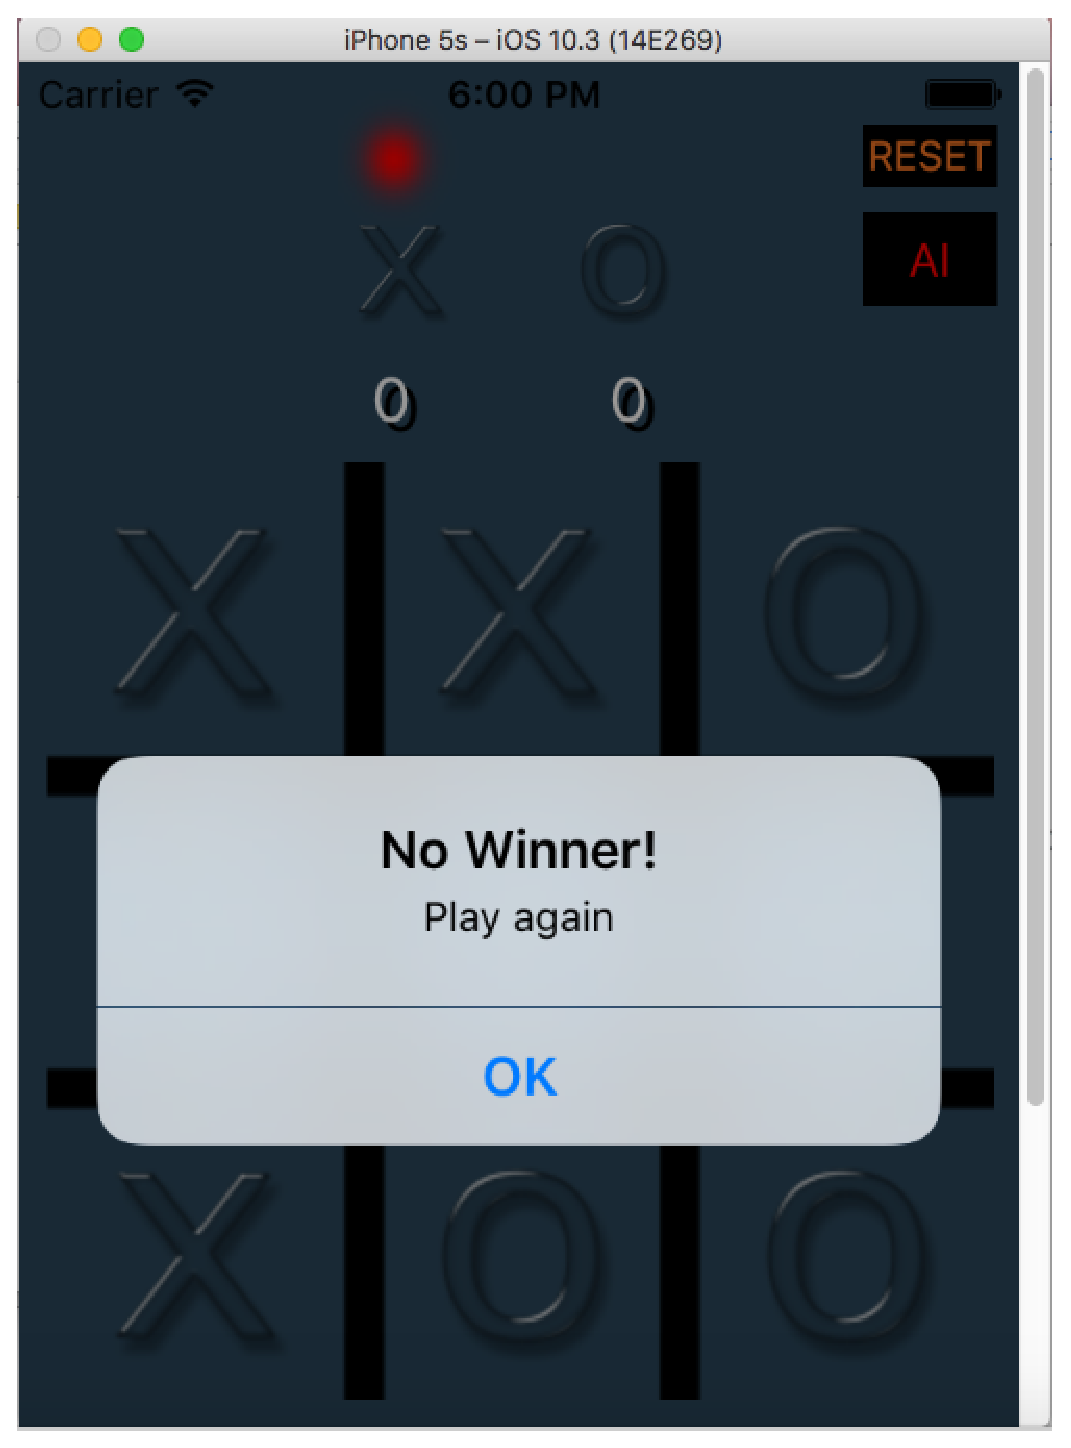
\includegraphics[width=\textwidth]{8.eps}\\
\\
Acum vom folosi comenzile descrise anterior.\\
\\
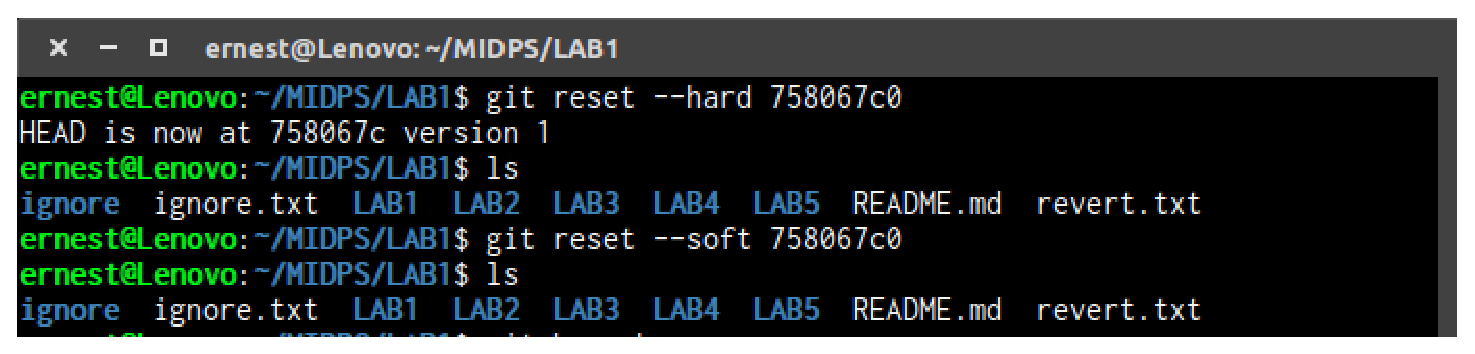
\includegraphics[width=\textwidth]{9.eps}\\
\\
Daca am facut niste schimbari in repozitoriu si nu ne satisfac, putem usor reveni
la ultima versiune care era pe git utilizind comanda \textbf{git pull origin "branch"}
